\section{Initial Ideas}
This task concerns itself with detecting two specific infrared frequencies to differentiate between the species of Wibbo and Snorkle. The first idea was just to test the phototransistor with no modifications whatsoever to gauge a sense of the accuracy. When the transistor was placed against the duck’s neck, our program detected frequencies which were outputted on our terminal, but they were sporadic and fluctuating between extreme values. Furthermore, at even a little distance away, signals could not be detected at all. The initial stance was therefore clear, we needed to amplify the signals from the phototransistor, and we needed to filter frequencies to get stable, accurate readings.

\section{Dissecting the Phototransistor}
\begin{figure}[h]
    \centering
    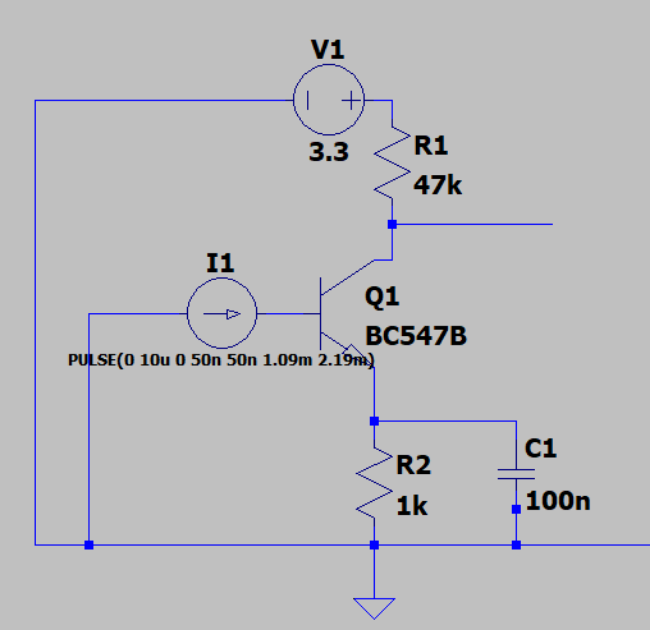
\includegraphics[width=0.8\textwidth]{subpages/images/phototransistor.png}
    \caption{The Phototransistor}
    \label{fig:phototransistor}
\end{figure}

The phototransistor is an electrical device that uses incoming light on its base and converts photons into electrons. By the photoelectric effect, light photons with adequate energy to exceed the work function excite electrons. This base current is amplified to produce a larger collector current. The design above mimics that of a common-emitter amplifier, where the wire drawn from the collector is to be amplified in the forthcoming stage.

The structure evident in Figure 2 involves an emitter degeneration resistor - as the emitter current rises, the voltage across Re rises and this in turn lowers the base-emitter voltage. This biases the transistor to prevent fluctuations in collector current and maintains thermal stability of the circuit. Biasing the input at Vbe is unwise given that several parameters vary with temperature. The negative feedback of the phototransistor ensures that the current generated stays within bounds.

The electrolytic capacitor boosts the gain by maintaining the biasing and attenuating AC signals. This introduces the low-pass filter for high-frequency noise early on to limit the frequencies we will be analysing.

A key adaptation is the pulse signal applied to the base. LTspice does not allow for simulation of light, but we are told that the duck emits pulses of infrared light. In Figure 3, the current source uses rise time and fall time of 50 nanoseconds with a full time-scope of 10 microseconds. Most importantly is the 2.19 millisecond period derived from the frequency of the 457Hz as period is the reciprocal of frequency - the pulse in LTspice mirrors the likely pulse emitted by the Wibbo.

\begin{figure}[h]
    \centering
    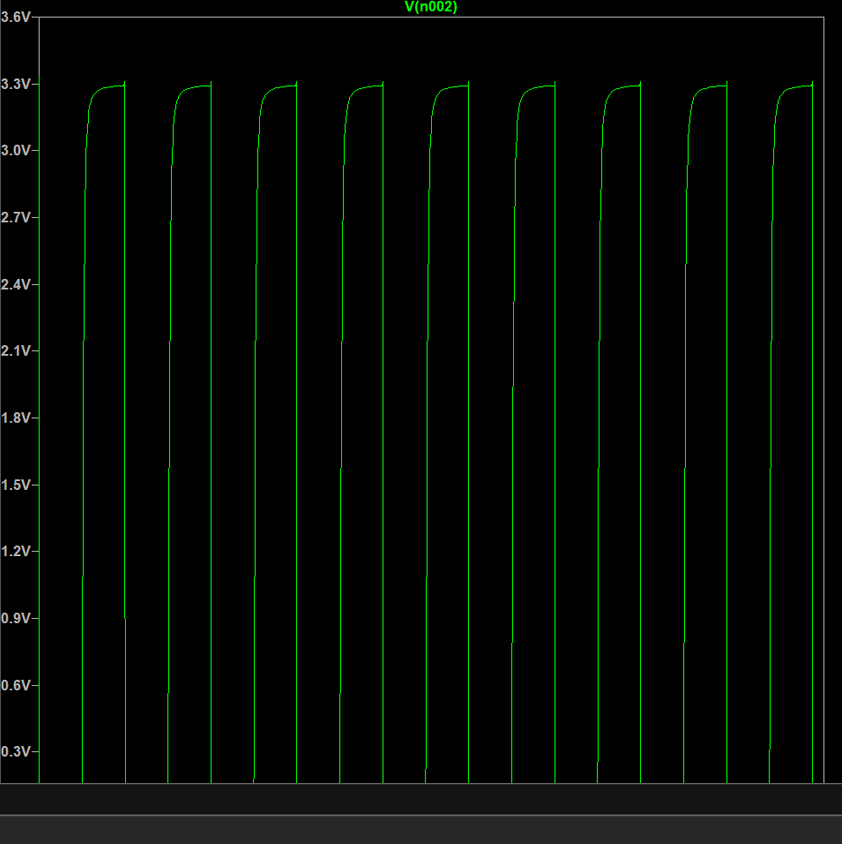
\includegraphics[width=0.8\textwidth]{subpages/images/pt_transient.png}
    \caption{Transient Analysis of Phototransistor}
    \label{fig:phototransistor_transient}
\end{figure}

Any transistor would be expected to amplify the signals it receives by set degree. Whilst the transient simulation above shows that the output voltage signal is square-like and around 3.3v amplitude which is what we desire – there are a couple of issues that deem this circuit inadmissible.

Issue 1: We are assuming that all the light directly hits the base when the light might scatter or potentially reflect meaning that our actual voltage output signal is far weaker.

Issue 2: Looking carefully at the peaks and troughs, we see that they do not perfectly mirror a square wave - there is overshooting and undershooting due to parasitic capacitance – a transistor in its switching process causes the voltage to stray from its bounds.

Issue 3: Though the waveform seems fine, there is an inverse relationship causing problems. When light hits the transistor, conduction causes the collector current to flow through the transistor to the ground. The voltage at the collector drops because the system sinks current. However, we would ideally prefer light hitting to cause a high voltage, so an inversion technique is required.

To ensure signals can be easily detected and follow correct logic, we must therefore consider the next phase of this design - the amplification stage.

\section{Amplification Analysis}
Following the phototransistor stage, the signal needs to be amplified given that it is currently too small for detection and may lead to our duck signals going under the radar. However, we also need to invert the waveform since the phototransistor operates under the basis of high light intensity leading to a low collector voltage. A non-inverting amplifier would result in a low pulse for the frequency detected and a high pulse for the light not detected. Whilst this remains easy to interpret, it is still inconvenient hence the need for our group to use an inverting amplifier as in Figure 4.4.

\begin{figure}[h]
    \centering
    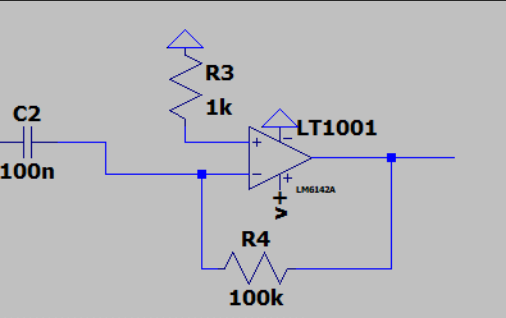
\includegraphics[width=0.8\textwidth]{subpages/images/amplification_stage.png}
    \caption{Transient Amplification Stage}
    \label{fig:amp_stage}
\end{figure}

Another component that has been added is the capacitor. This acts as a filter to attenuate ambient light changes but more importantly, remove DC bias. Selecting too high of a capacitance would increase the time constant and longer discharging would cause lag to the pulses.

To ensure clear detection, we have used a feedback resistor of 100k and a Rin of 1k to give a gain of -100. This helps us achieve the correct waveform pattern and ensures the voltages are sufficient for detection, especially when the ducks stray further from the infrared detector system.

\section{Complexities using Band-Pass Filters}
With the amplification side completed, we now needed to closely inspect the frequencies we are after. For this, there were several filters to consider but through this sub-section, we will reach an interesting conclusion.

First, we considered the passive filters and targeted a bandpass filter, depicted in Figure 5, as a standard low-pass filter or high-pass filter would not be sufficient. The bandpass is not between the Snorkle and Wibbo frequencies but rather the limits are set by our acceptable range for each frequency should it deviate. A Wibbo has 457Hz, so we set a 10Hz allowance either side and set the cutoff frequencies as 447 and 467 during the simulations demonstrated in Figure 4.6.

\begin{figure}[h]
    \centering
    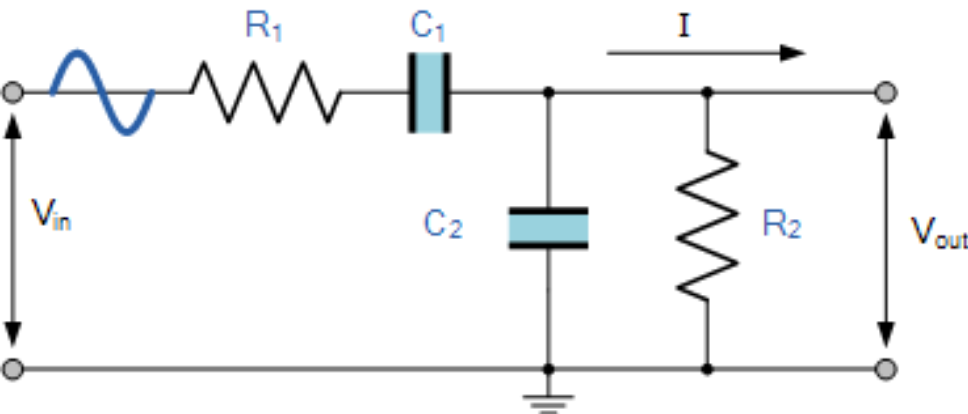
\includegraphics[width=0.8\textwidth]{subpages/images/passive_bp_filter.png}
    \caption{Passive Band-Pass Filter}
    \label{fig:passive_bp_filter}
\end{figure}
\begin{figure}[h]
    \centering
    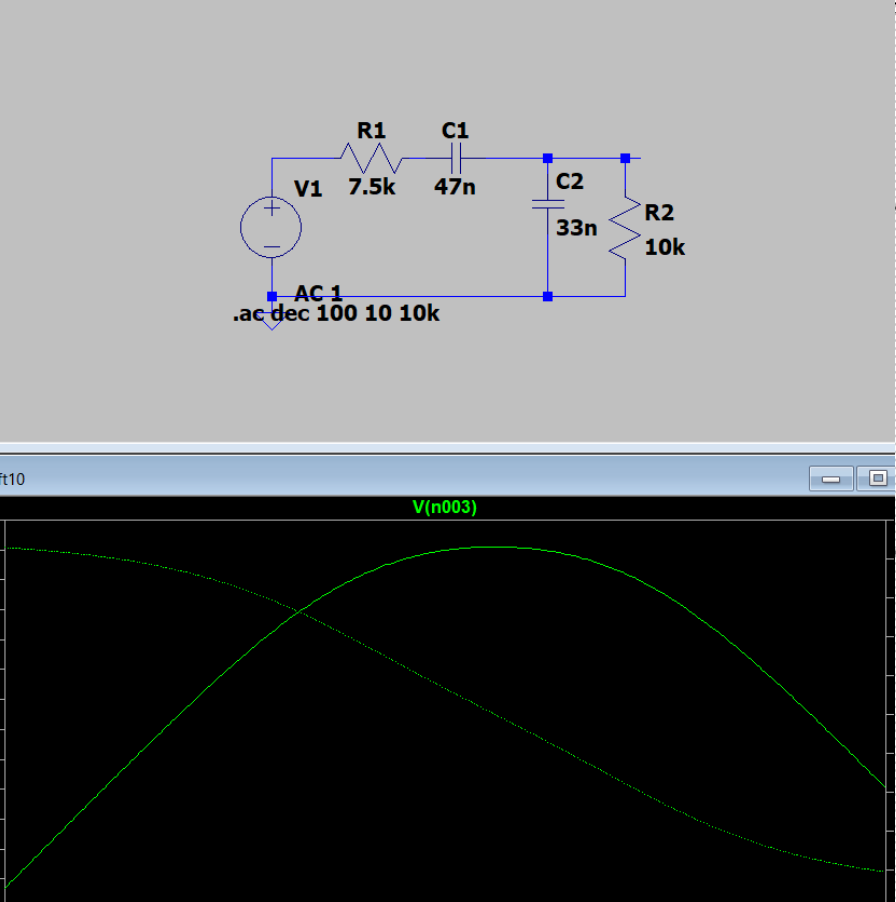
\includegraphics[width=0.8\textwidth]{subpages/images/test_passive_bp.png}
    \caption{Testing Passive Band-Pass Filter}
    \label{fig:passive_bp_filter}
\end{figure}

The calculations are as followed for the high-pass and low-pass filters.
\begin{enumerate}
    \item High-Pass Filter
          The cut-off frequency is given by \(f_c = \frac{1}{2\pi RC}\).
          For our values, R = 7.5k$\Omega$ and C = 47nF, this gives a cut-off at approximately 451.2Hz, which is within 0.94\% of the target 447Hz.
    \item Low-Pass Filter
          We have values R = 10k$\Omega$ and C = 33nF. This gives a cut-off at approximately 482.8Hz. This is is within 3.39\% of the target 467Hz.
\end{enumerate}

However, whilst passive filters are simpler and require less power, they cannot provide gain and rely on large inductor and capacitor values to function effectively. These components dissipate more energy near resonance, and such losses reduce the system's ability to sustain resonance.
\begin{itemize}
    \item A low Q means the circuit does not respond strongly to its natural frequency.
    \item Therefore, the filter allows a broad range of frequencies near the cutoff
    \item This results in a non-sharp cutoff; the transition from passband to stopband is gradual, not steep.
    \item Without amplification, any small energy losses cannot be corrected, meaning the filter is not sharply selective.
\end{itemize}

\begin{figure}[h]
    \centering
    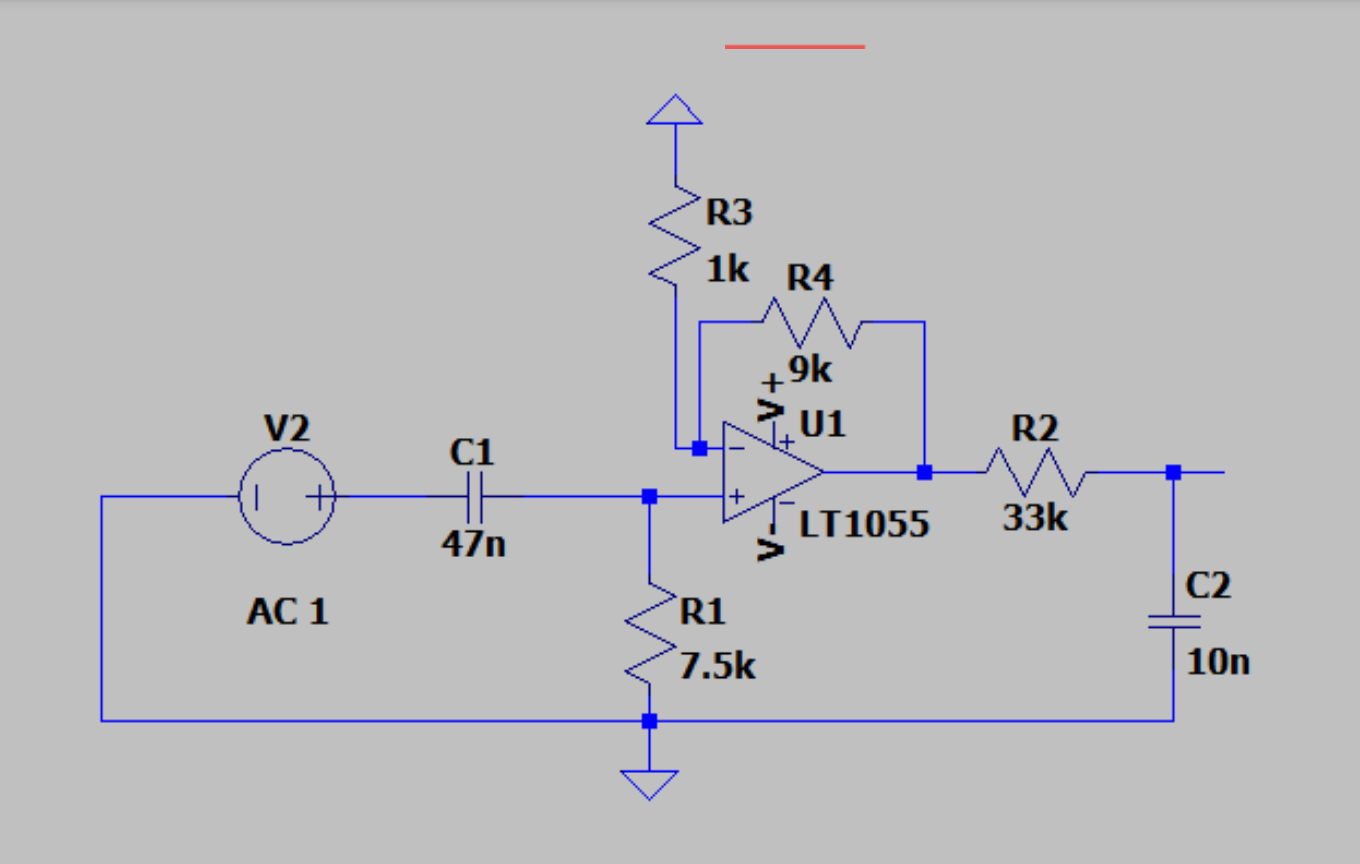
\includegraphics[width=0.8\textwidth]{subpages/images/non-invert-active-bp-filter.png}
    \caption{Non-Inverting Active Band-Pass Filter}
    \label{fig:active_bp_filter}
\end{figure}
\begin{figure}[h]
    \centering
    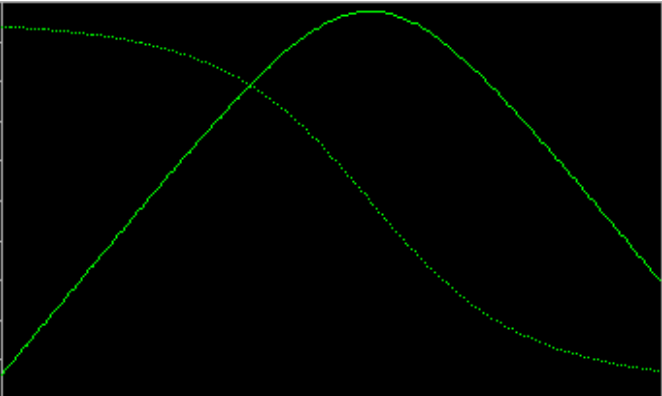
\includegraphics[width=0.8\textwidth]{subpages/images/ir_result_1.png}
    \caption{Simulation Results}
    \label{fig:simul_result}
\end{figure}

The circuit in Figure 4.6 represents a non-inverting active band-pass filter re-using the components calculated from earlier but now including an op-amp. We have the high-pass filter first, then the amplification and finally the low-pass filter. R3 and R4 also work together to give us a gain of 10 - calculated by \(1+ \frac{R_f}{R_{In}} \) - which is reasonable and can always be adjusted if there is clipping.

Though we would expect a flat band-pass, we have also picked quite a narrow range for the cutoff frequencies - hence why the AC sweep in Figure 10 shows the right peak at 20dB but a swift rise and fall.

The last strategy was the Sallen-Key band-pass filter. The second-order filter can be precisely tuned using resistor and capacitors, leading to a potential symmetrical bell-shaped response for AC sweep. It also involves positive and negative feedback to shape the frequency. However, as clear below in figure 4.8, the circuitry becomes quite overwhelming.

\begin{figure}[h]
    \centering
    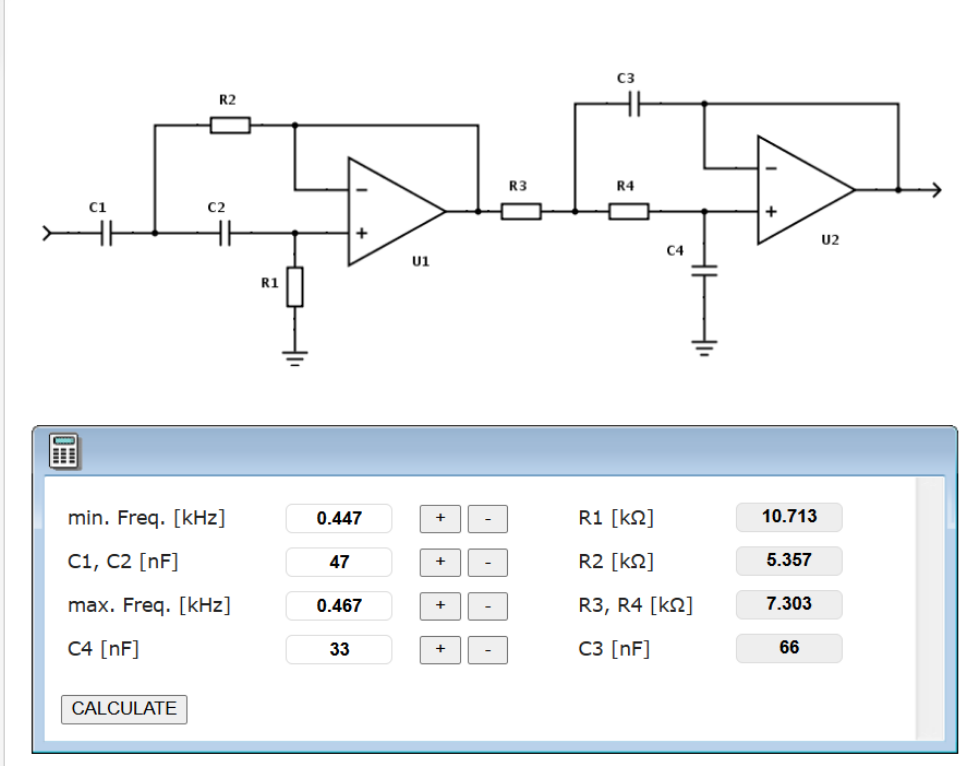
\includegraphics[width=0.8\textwidth]{subpages/images/sallen_key.png}
    \caption{Sallen-Key Analysis 1}
    \label{fig:sallen_key}
\end{figure}

The following simulation on LTspice show the peak frequency at around 458Hz and our target for the Wibbo was 457Hz implying that the Sallen-Key is filtering correctly and provides a nice bell-shaped symmetrical frequency response.

\begin{figure}[h]
    \centering
    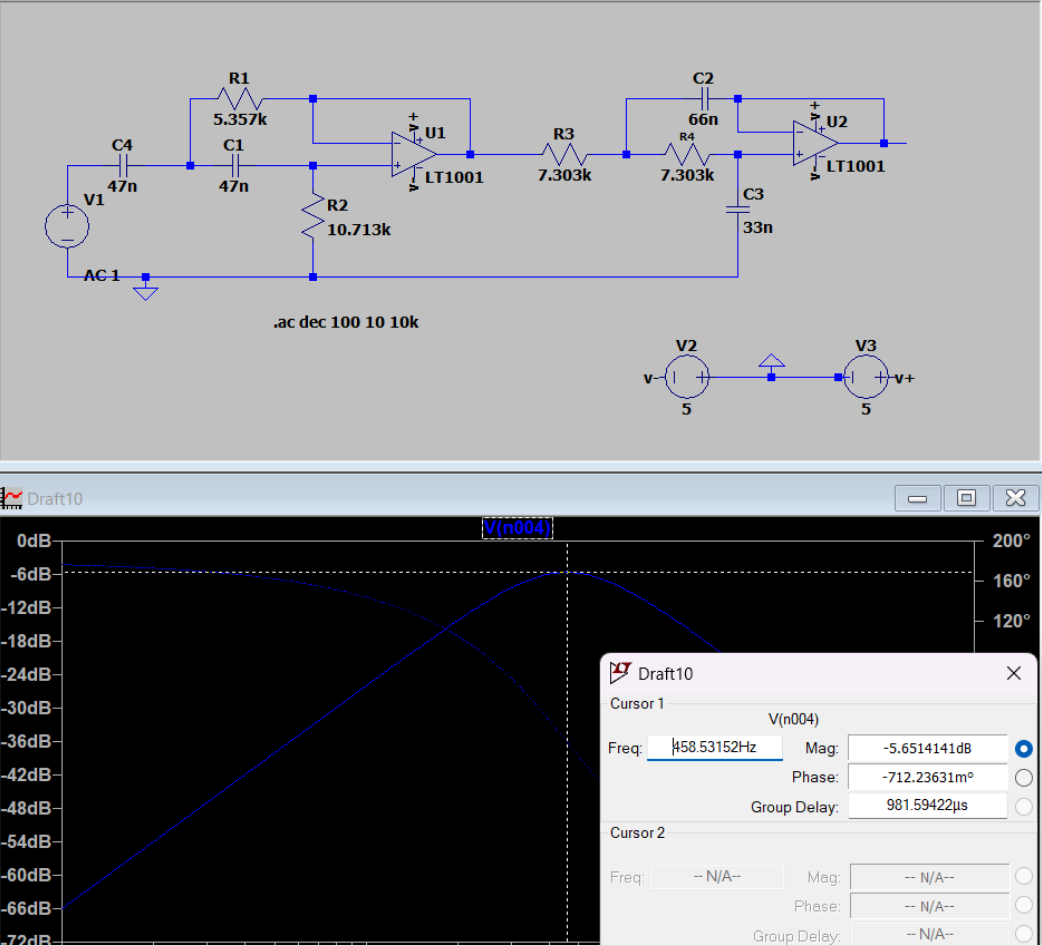
\includegraphics[width=0.8\textwidth]{subpages/images/sallen_key2.png}
    \caption{Sallen-Key Analysis 2}
    \label{fig:sallen_key2}
\end{figure}

Despite this, the issue should be clear by now. We need to utilise two band-pass filters to account for both Wibbo detection and Snorkle detection, which will make this circuit severely complicated. When using LTspice, the final hypothetical circuit would look like the diagram on the next page.

Following this, the conclusion was that hardware was going to take up space and get complicated very quickly. To mitigate the complexities, we needed to think of a method that took less time, not as complicated and helped us get the frequencies we needed. The solution to this was turning to our Arduino code.
\begin{figure}[H]
    \centering
    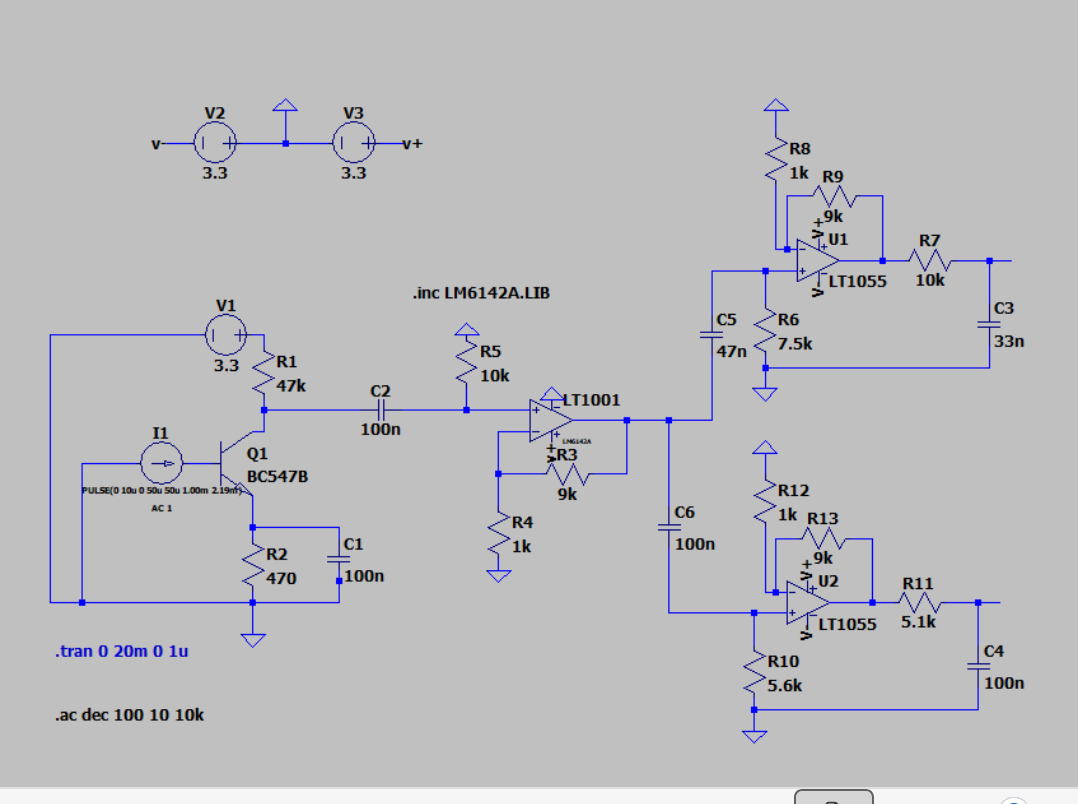
\includegraphics[width=0.8\textwidth]{subpages/images/ir_complex.png}
    \caption{Complete Circuit Diagram - For Analysis Only}
    \label{fig:complex_circuit}
\end{figure}

Before that, another sidenote would be the selection of the LM324N operational amplifier. Whilst alternatives like ADA4817 and OPA3333 were evaluated for their higher bandwidth, lower noise, and favourable slew rate, they were both surface mounted. This means they sit on a PCB and do not have flexible leads which, on top of being exceedingly small, make them difficult to work and test with plus if damaged could harm our budgeting.

The LM324N offers an output swing between -1.5v to 1.5v with a 5v single supply which preserves signals, without clipping, even at extremely low supply voltages. Furthermore, the infrared pulses that hit the phototransistor will produce weak transient signals that require amplification without distorting harmonies. The gain-bandwidth product for this op-amp is 1MHz meaning that for the short pulses, which contain a multitude of frequency components beyond the fundamental, this modest GBP can ensure the op-amp maintains signal integrity and effectively manages the signal bandwidth during said amplification.

Noise performance also represents a critical consideration in the characteristics of this op-amp. The LM324N exhibits an input bias current of 45nA with temperature compensation, and an input offset voltage of just 2mV. While these specifications may not complete match the requirements of precision amplifiers, they prove sufficient given the signal levels being dealt with.

The selected op-amp also demonstrates excellent phase margin characteristics, maintaining stability even when driving capacitive loads at the output stage. This robustness against oscillation ensures clean, undistorted signal regeneration without the need for further, complicated stabilization networks.

Thus, though trade-offs were required, the LM324N presented itself most favourable for this detection system and depicted below for practical reference.

\begin{figure}[H]
    \centering
    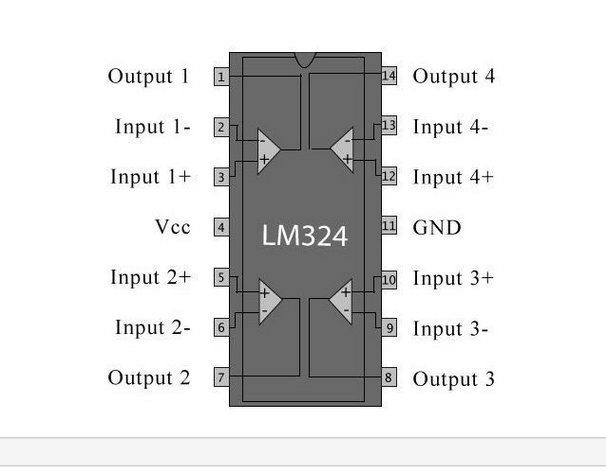
\includegraphics[width=0.8\textwidth]{subpages/images/lm324n.png}
    \caption{LM324N Cross-Section}
    \label{fig:lm324n}
\end{figure}

\section{Simplification using Arduino}
After discussing with a member of staff, Dr Hakan Merdan, the team unanimously agreed that there was a way to manipulate the Arduino code to our advantage. Though the full, updated code will be discussed later, the following snapshot depicts an earlier version of this key section.
\begin{verbatim}
// Check for Wibbo: 447-467Hz
if (frequency >= 447 && frequency <= 470) {
    response += "It's a Wibbo!";
}
// Check for Snorkle: up to 303Hz
else if (frequency >= 283 && frequency <= 303) {
    response += "It's a Snorkle!";
}
\end{verbatim}
Our original method of analogue filtering involved two band-pass filters which would avoid software processing delays and identify species well, but the circuitry is complex, has limited flexibility and components can be very sensitive.

Our upgraded method of digital signal processing uses \texttt{pulseIn()} to measure high/low amplified phototransistor signals. The following line:
\begin{verbatim}
float frequency = 1000000.0 / (highTime + lowTime)
\end{verbatim}
calculates the frequency of the pulses mathematically while the snapshot above compares against the expected range. Note that we have not targeted the specific species-related frequency but instead allowed for a range due to deviations in the signal frequency.

This tactic involves simpler hardware, reduced space and weight, flexible thresholds using small change in code and no risk of errors due to parasitic impedance or capacitance of components. However, software implementation does possess limitations such as timing inaccuracies when handling multiple asynchronous sensor inputs. With several sensors sending data that the Arduino needs to read and interpret, the interface may experience a slight lag.

Our final circuit -- with no filters and output to be connected to our Metro M0 microcontroller -- therefore looks like this with the supporting transient simulation:
\begin{figure}[h]
    \centering
    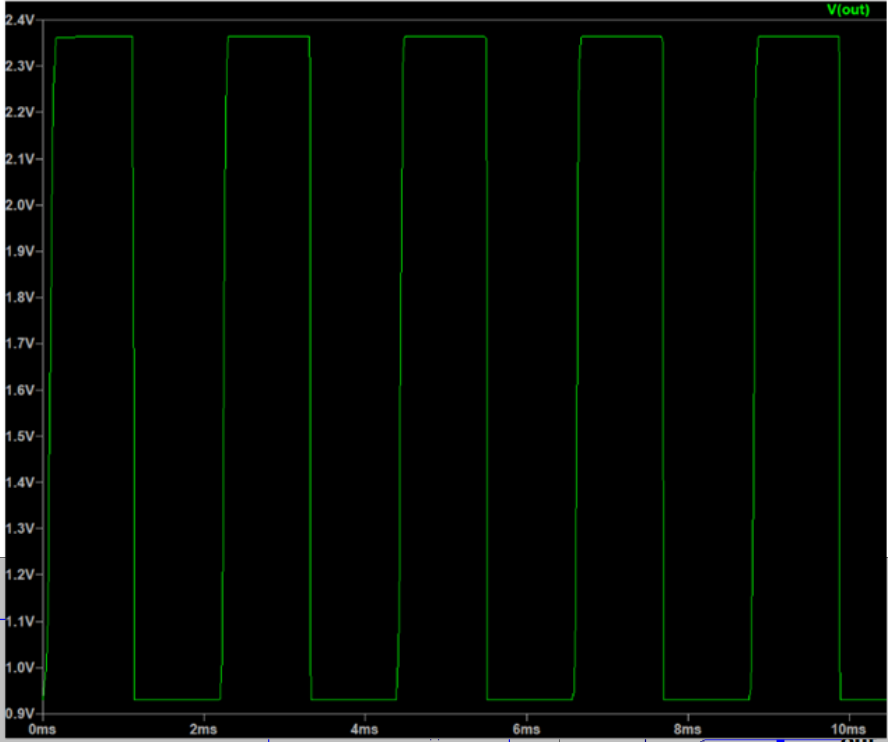
\includegraphics[width=0.8\textwidth]{subpages/images/ir_expected.png}
    \caption{Expected Results from Simulation}
    \label{fig:expected_results}
\end{figure}
\begin{figure}[h]
    \centering
    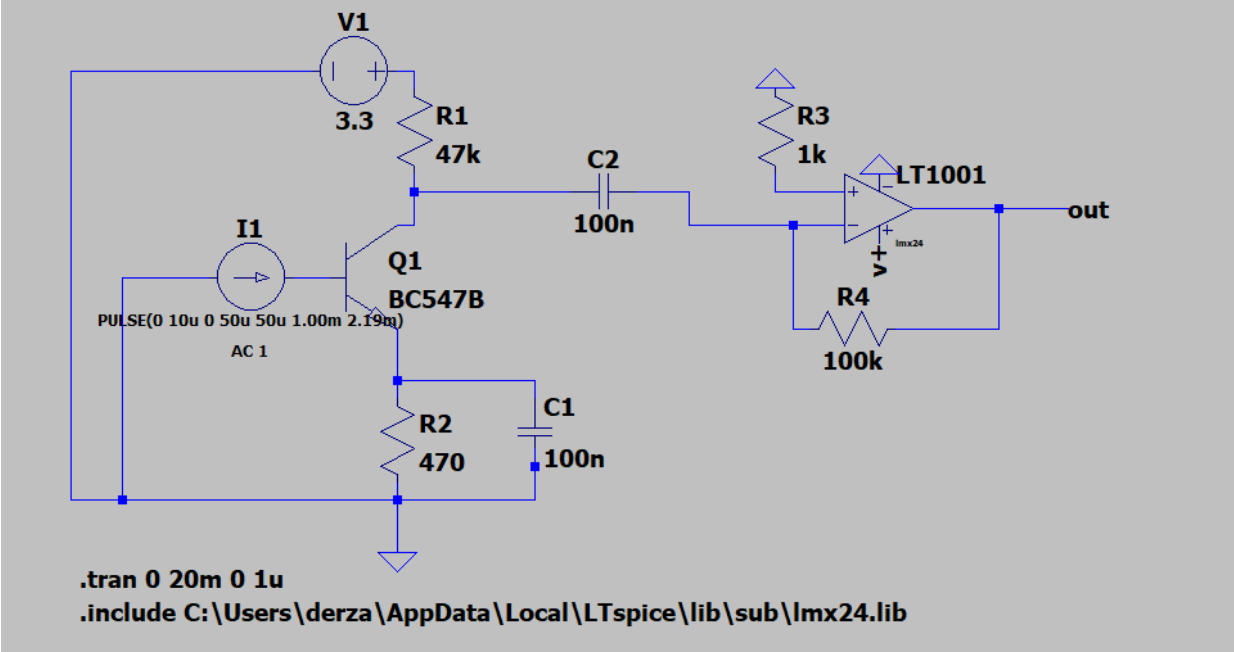
\includegraphics[width=0.8\textwidth]{subpages/images/ir_final.png}
    \caption{Final SPICE Circuit for IR Detection}
    \label{fig:final_circuit}
\end{figure}

The procedure flowchart below clearly summarizes the steps that have and will be taken in this Infrared Detection task.
\begin{figure}[h]
    \centering
    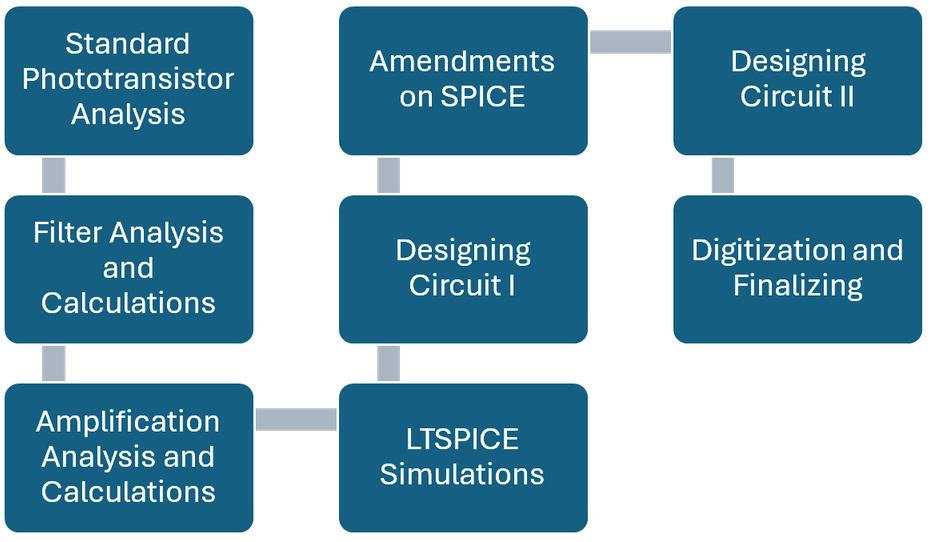
\includegraphics[width=0.8\textwidth]{subpages/images/ir_procedure.png}
    \caption{Infrared Detection Task Flowchart}
    \label{fig:ir_flowchart}
\end{figure}
\begin{figure}[h]
    \centering
    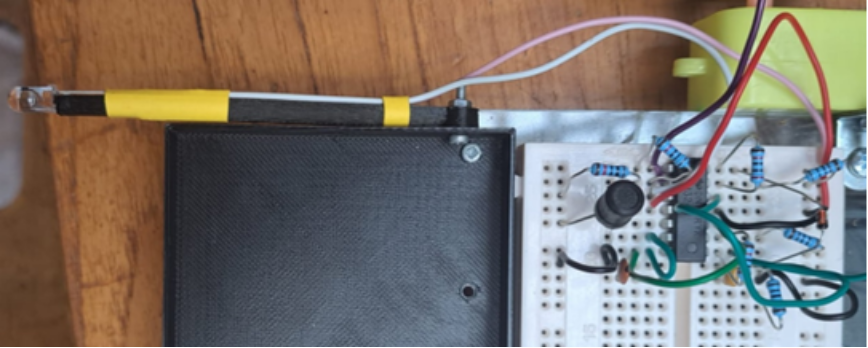
\includegraphics[width=0.8\textwidth]{subpages/images/ir_irl.png}
    \caption{IR Circuit}
    \label{fig:ir_circuit}
\end{figure}

\section{Building and Testing}
The breadboard circuit constructed led to successful practical simulation where the sharp pulses were detected on this oscilloscope. Evidently, these pulses starkly contrast the square pulses we expected from the SPICE simulation. In real hardware, the IR light from the ducks is emitted in sharp bursts compared to perfectly square waveforms. Building on this, the phototransistor response is rapid and therefore the oscilloscope showed the narrowest part of the signal. Other reasons could have been the bandwidth limits compressing the rising and falling edges into narrower spikes.
\begin{figure}[h]
    \centering
    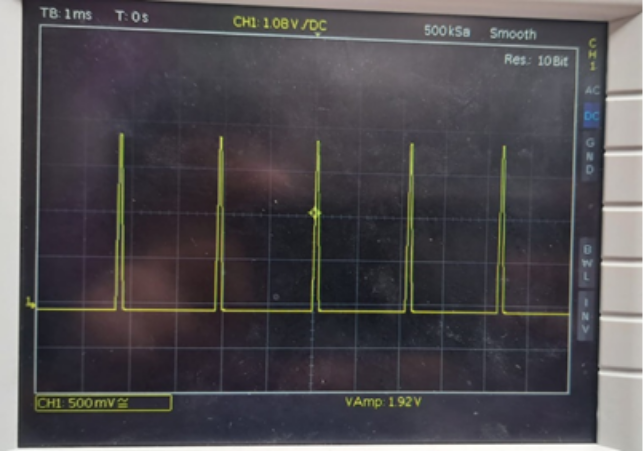
\includegraphics[width=0.8\textwidth]{subpages/images/ir_probe.png}
    \caption{Results for Probing IR Circuit}
    \label{fig:ir_probe}
\end{figure}

Regardless, the pulses in Figure 4.16 are still exhibited when the phototransistor is within reasonable proximity of the ducks leading to our interface correctly outputting the species and respective frequency.

However, initial analysis revealed that there was a minor inconvenience to our detector. Whilst the IR light was detected at a sufficient distance, the pulses were far weaker at first. This result contradicted the idea of amplification and led to circuit checks which were to no avail. Eventually, it became apparent that when there was a cover over the transistor, the pulses are as seen in the image but weaker and less clear when completely exposed. The ambient light from the room was most likely interfering because whilst we have digitally filtered the frequencies, the oscilloscope-probing process is independent of that. Hence, this led into the next step – design a cover to ensure other frequencies are not interfering with our IR detector.

With the desired signal, the detection system is complete for the Wibbo and Snorkle species. This was an example of species detection which will be returned to, but the next section concerns itself with name identification.
